\documentclass[english,floatsintext,man]{apa6}

\usepackage{amssymb,amsmath}
\usepackage{ifxetex,ifluatex}
\usepackage{fixltx2e} % provides \textsubscript
\ifnum 0\ifxetex 1\fi\ifluatex 1\fi=0 % if pdftex
  \usepackage[T1]{fontenc}
  \usepackage[utf8]{inputenc}
\else % if luatex or xelatex
  \ifxetex
    \usepackage{mathspec}
    \usepackage{xltxtra,xunicode}
  \else
    \usepackage{fontspec}
  \fi
  \defaultfontfeatures{Mapping=tex-text,Scale=MatchLowercase}
  \newcommand{\euro}{€}
\fi
% use upquote if available, for straight quotes in verbatim environments
\IfFileExists{upquote.sty}{\usepackage{upquote}}{}
% use microtype if available
\IfFileExists{microtype.sty}{\usepackage{microtype}}{}

% Table formatting
\usepackage{longtable, booktabs}
\usepackage{lscape}
% \usepackage[counterclockwise]{rotating}   % Landscape page setup for large tables
\usepackage{multirow}		% Table styling
\usepackage{tabularx}		% Control Column width
\usepackage[flushleft]{threeparttable}	% Allows for three part tables with a specified notes section
\usepackage{threeparttablex}            % Lets threeparttable work with longtable

% Create new environments so endfloat can handle them
% \newenvironment{ltable}
%   {\begin{landscape}\begin{center}\begin{threeparttable}}
%   {\end{threeparttable}\end{center}\end{landscape}}

\newenvironment{lltable}
  {\begin{landscape}\begin{center}\begin{ThreePartTable}}
  {\end{ThreePartTable}\end{center}\end{landscape}}




% The following enables adjusting longtable caption width to table width
% Solution found at http://golatex.de/longtable-mit-caption-so-breit-wie-die-tabelle-t15767.html
\makeatletter
\newcommand\LastLTentrywidth{1em}
\newlength\longtablewidth
\setlength{\longtablewidth}{1in}
\newcommand\getlongtablewidth{%
 \begingroup
  \ifcsname LT@\roman{LT@tables}\endcsname
  \global\longtablewidth=0pt
  \renewcommand\LT@entry[2]{\global\advance\longtablewidth by ##2\relax\gdef\LastLTentrywidth{##2}}%
  \@nameuse{LT@\roman{LT@tables}}%
  \fi
\endgroup}


  \usepackage{graphicx}
  \makeatletter
  \def\maxwidth{\ifdim\Gin@nat@width>\linewidth\linewidth\else\Gin@nat@width\fi}
  \def\maxheight{\ifdim\Gin@nat@height>\textheight\textheight\else\Gin@nat@height\fi}
  \makeatother
  % Scale images if necessary, so that they will not overflow the page
  % margins by default, and it is still possible to overwrite the defaults
  % using explicit options in \includegraphics[width, height, ...]{}
  \setkeys{Gin}{width=\maxwidth,height=\maxheight,keepaspectratio}
\ifxetex
  \usepackage[setpagesize=false, % page size defined by xetex
              unicode=false, % unicode breaks when used with xetex
              xetex]{hyperref}
\else
  \usepackage[unicode=true]{hyperref}
\fi
\hypersetup{breaklinks=true,
            pdfauthor={},
            pdftitle={The emergence of words from vocal imitations},
            colorlinks=true,
            citecolor=blue,
            urlcolor=blue,
            linkcolor=black,
            pdfborder={0 0 0}}
\urlstyle{same}  % don't use monospace font for urls

\setlength{\parindent}{0pt}
%\setlength{\parskip}{0pt plus 0pt minus 0pt}

\setlength{\emergencystretch}{3em}  % prevent overfull lines

\ifxetex
  \usepackage{polyglossia}
  \setmainlanguage{}
\else
  \usepackage[english]{babel}
\fi

% Manuscript styling
\captionsetup{font=singlespacing,justification=justified}
\usepackage{csquotes}
\usepackage{upgreek}

 % Line numbering
  \usepackage{lineno}
  \linenumbers


\usepackage{tikz} % Variable definition to generate author note

% fix for \tightlist problem in pandoc 1.14
\providecommand{\tightlist}{%
  \setlength{\itemsep}{0pt}\setlength{\parskip}{0pt}}

% Essential manuscript parts
  \title{The emergence of words from vocal imitations}

  \shorttitle{Words from imitations}


  \author{Pierce Edmiston\textsuperscript{1}, Marcus Perlman\textsuperscript{2}, \& Gary Lupyan\textsuperscript{1}}

  % \def\affdep{{"", "", ""}}%
  % \def\affcity{{"", "", ""}}%

  \affiliation{
    \vspace{0.5cm}
          \textsuperscript{1} University of Wisconsin-Madison\\
          \textsuperscript{2} University of Birmingham  }

  \authornote{
    Pierce Edmiston and Gary Lupyan, Department of Psychology, University of
    Wisconsin-Madison, Madison, Wisconsin. Marcus Perlman, Department of
    English Language and Applied Linguistics, University of Birmingham,
    United Kingdom.
    
    Correspondence concerning this article should be addressed to Pierce
    Edmiston, 1202 W. Johnson St., Madison, WI, 53703. E-mail:
    \href{mailto:pedmiston@wisc.edu}{\nolinkurl{pedmiston@wisc.edu}}
  }


  \abstract{People have long pondered the origins of language, especially the words
that compose them. Here, we report a series of experiments investigating
how conventional spoken words might emerge from imitations of
environmental sounds. Does the repeated imitation of an environmental
sound gradually give rise to more word-like forms? In what ways do these
words resemble the original sounds that motivated them (i.e.,
iconicity)? Participants played a version of the children's game
``Telephone''. The first generation of participants imitated
recognizable environmental sounds (e.g., glass breaking, water
splashing). Subsequent generations imitated the previous generation of
imitations for a maximum of 8 generations. The results showed that the
imitations became more stable and word-like, and later imitations were
easier to learn as category labels. At the same time, even after 8
generations, both spoken imitations and their written transcriptions
could be matched above chance to the category of environmental sound
that motivated them. These results show how repeated imitation can
create progressively more word-like forms while continuing to retain a
resemblance to the original sound that motivated them, and speak to the
possible role of human vocal imitation in explaining the origins of at
least some spoken words.}
  \keywords{language evolution, iconicity, vocal imitation, transmission chain \\

    \indent Word count: 6913
  }

\usepackage[titles]{tocloft}
\cftpagenumbersoff{figure}
\renewcommand{\cftfigpresnum}{\itshape\figurename\enspace}
\renewcommand{\cftfigaftersnum}{.\space}
\setlength{\cftfigindent}{0pt}
\setlength{\cftafterloftitleskip}{0pt}
\settowidth{\cftfignumwidth}{Figure 10.\qquad}

\cftpagenumbersoff{table}
\renewcommand{\cfttabpresnum}{\itshape\tablename\enspace}
\renewcommand{\cfttabaftersnum}{.\space}
\setlength{\cfttabindent}{0pt}
\setlength{\cftafterloftitleskip}{0pt}
\settowidth{\cfttabnumwidth}{Table 10.\qquad}



\usepackage{amsthm}
\newtheorem{theorem}{Theorem}
\newtheorem{lemma}{Lemma}
\theoremstyle{definition}
\newtheorem{definition}{Definition}
\newtheorem{corollary}{Corollary}
\newtheorem{proposition}{Proposition}
\theoremstyle{definition}
\newtheorem{example}{Example}
\theoremstyle{definition}
\newtheorem{exercise}{Exercise}
\theoremstyle{remark}
\newtheorem*{remark}{Remark}
\newtheorem*{solution}{Solution}
\begin{document}

\maketitle

\setcounter{secnumdepth}{0}



Most vocal communication of non-human primate species is based on
species-typical calls that are highly similar across generations and
between populations {[}1{]} {[}2{]}. In contrast, human languages
comprise a vast repertoire of learned meaningful elements (words and
other morphemes) which can number in the tens of thousands or more
{[}3{]}. Aside from their number, the words of different natural
languages are characterized by their extreme diversity {[}4--6{]}. The
words used within a speech community change relatively quickly over
generations compared to the evolution of vocal signals {[}7{]}. At least
in part as a consequence of this divergence, most words appear to bear a
largely arbitrary relationship between their form and their meaning ---
seemingly, a product of their idiosyncratic etymological histories
{[}8,9{]}. The apparently arbitrary nature of spoken vocabularies
presents a quandary for the study of language origins. If words of
spoken languages are truly arbitrary, by what process were the first
words ever coined?

While the origin of most spoken words is hard to discern, the situation
is somewhat different for signed languages. In signed languages, the
origins of many signs are relatively transparent. Although signed
languages rely on the same type of referential symbolism as spoken
languages, many individual signs have clear iconic roots, formed from
gestures that resemble their meaning {[}10--12{]}. For instance,
{[}13{]} noted the iconic origins of the American Sign Language (ASL)
sign for bird, which is formed with a beak-like handshape articulated in
front of the nose. Another example is steal, derived from a grabbing
motion to represent the act of stealing something. {[}14{]} identified
about 25\% of American Sign Language signs to be iconic, and reviewing
the remaining 75\% of ASL signs, {[}15{]} determined that about
two-thirds of these seemed plausibly derived from iconic origins.
Further support for iconic origins of signed languages comes from
observations of deaf children raised without exposure to a signed
language, who develop homesign systems to use with their family. These
communication systems are generally built from a process in which the
children establish conventional gestures through the use of pantomimes
and various iconic and indexical gestures {[}16{]}. Participants in
laboratory experiments utilize a similar strategy when they communicate
with gestures in iterated communication games {[}17{]}.

In contrast to the visual gestures of signed languages, many have argued
that iconic vocalizations could not have played a significant role in
the origin of spoken words because the vocal modality simply does not
afford much resemblance between form and meaning {[}18--23{]}. It has
also been argued that the human capacity for vocal imitation is a
domain-specific skill, geared towards learning to speak, rather than the
representation of environmental sounds. For example, {[}24{]} suggested
that, \enquote{most humans lack the ability\ldots{} to convincingly
reproduce environmental sounds\ldots{} Thus \enquote{capacity for vocal
imitation} in humans might be better described as a capacity to learn to
produce speech} (p.~209). Consequently, it is still widely assumed that
vocal imitation --- or more broadly, the use of any sort of resemblance
between form and meaning --- cannot be important to understanding the
origin of spoken words.

Although most words of contemporary spoken languages are not clearly
imitative in origin, there has been a growing recognition of the
importance of iconicity in spoken languages {[}25,26{]} and the common
use of vocal imitation and depiction in spoken discourse {[}27,28{]}.
This has led some to argue for the importance of imitation for
understanding the origin of spoken words {[}29--33{]}. In addition,
counter to previous assumptions, people are highly effective at using
vocal imitations to refer to environmental sounds such as coins dropping
in a jar or mechanical events such as scraping --- in some cases, even
more effective than when using conventional words {[}34{]}. Recent work
has also shown that people are able to create novel imitative
vocalizations for more abstract meanings (e.g. \enquote{slow},
\enquote{rough}, \enquote{good}, \enquote{many}) that are understandable
to naïve listeners {[}33{]}. These imitations are effective not because
people can mimic environmental sounds with high fidelity, but because
people are able to produce imitations that capture the salient features
of sounds in ways that are understandable to listeners {[}35{]}.
Similarly, the features of onomatopoeic words might highlight
distinctive aspects of the sounds they represent. For example, the
initial voiced, plosive /b/ in \enquote{boom} represents an abrupt, loud
onset, the back vowel /u/ a low pitch, and the nasalized /m/ a slow,
muffled decay {[}36{]}.

Thus, converging evidence suggests that people can use vocal imitation
as an effective means of communication. At the same time, vocal
imitations are not words. If vocal imitation played a role in the origin
of some spoken words, then it is necessary to identify the minimal
conditions under which vocal imitations can give rise to more word-like
vocalizations that can eventually be integrated into a vocabulary of a
language. In the present set of studies we ask whether vocal imitations
can transition to more word-like forms through sheer repetition ---
without an explicit intent to communicate. To answer this question, we
recruited participants to play an online version of the children's game
of \enquote{Telephone}. In the children's game, a spoken message is
whispered from one person to the next. In our version, the original
message or \enquote{seed sound} was a recording of an environmental
sound. The initial group of participants (first generation) imitated
these seed sounds, the next generation imitated the previous imitators,
and so on for up to 8 generations.

Our approach uses a transmission chain methodology similar to that
frequently used in experimental studies of language evolution {[}37{]}.
As with other transmission chain studies (and iterated learning studies
more generally), we seek to discover how various biases and constraints
of individuals change the nature of a linguistic signal. Importantly,
while typical transmission chain studies focus on the impact of learning
biases {[}38{]}, the present studies involve iterated reproduction that
does not involve any learning. Participants simply attempt to imitate a
sound as best as they can. The biases we hypothesize to drive
vocalizations to become more word-like are therefore not related to any
learning process, but instead are expected to emerge from constraints on
the reproducibility of vocalizations. Our aim is thus to determine
whether iterated reproduction, even without learning, is a sufficient
enough constraint to enable the emergence of more word-like signals.

After collecting the imitations, we conducted a series of analyses and
additional experiments to systematically answer the following questions:
First, do imitations stabilize in form and become more word-like as they
are repeated? Second, do the imitations retain a resemblance to the
original environmental sound that inspired them? If so, it should be
possible for naïve participants to match the emergent words back to the
original seed sounds. Third, do the imitations become more suitable as
categorical labels for the sounds that motivated them? For example, does
the imitation of a particular water-splashing sound become, over
generations of repeated imitation, a better label for the more general
category of water-splashing sounds?

\hypertarget{experiment-1-stabilization-of-imitations-through-repetition}{%
\section{Experiment 1: Stabilization of imitations through
repetition}\label{experiment-1-stabilization-of-imitations-through-repetition}}

In the first experiment, we collected the vocal imitations, and assessed
the extent to which repeating imitations of environmental sounds results
in progressive stabilization toward more word-like forms in three ways.
First, we measured changes in the perception of acoustic similarity
between subsequent generations of imitations. Second, we used
algorithmic measures of acoustic similarity to assess the similarity of
imitations sampled within and between transmission chains. Third, we
obtained transcriptions of imitations, and measured the extent to which
later generation imitations were transcribed with greater consistency
and agreement. The results show that repeated imitation results in
vocalizations that are easier to repeat with high fidelity and more
consistently transcribed into English orthography.

\hypertarget{methods}{%
\subsection{Methods}\label{methods}}

\hypertarget{selecting-seed-sounds}{%
\subsubsection{Selecting seed sounds}\label{selecting-seed-sounds}}

To avoid sounds with lexicalized or conventionalized onomatopoeic forms
in English, we used inanimate categories of environmental sounds. To
select sounds that were equally distinguishable within each category, we
used an odd-one-out norming procedure (\emph{N}=105 participants; see
Fig. S1), resulting in a final set of 16 sounds, 4 in each of 4
categories: glass, tear, water, zipper.

\hypertarget{collecting-vocal-imitations}{%
\subsubsection{Collecting vocal
imitations}\label{collecting-vocal-imitations}}

Participants (\emph{N}=94) recruited from Amazon Mechanical Turk were
paid to participate in an online version of the children's game of
\enquote{Telephone}. Participants were instructed that they would hear
some sound and their task was to reproduce it as accurately as possible
using their computer microphone. Full instructions are provided in the
Supplemental Materials.

Each participant listened to and imitated four sounds: one from each of
the four categories of environmental sounds. Sounds were assigned at
random such that participants were unlikely to imitate the same person
more than once. Participants were allowed to listen to each target sound
as many times as they wished, but were only allowed a single recording
in response. Recordings that were too quiet (less than -30 dBFS) were
not accepted.

Imitations were monitored by an experimenter to remove poor quality
recordings (e.g., loud background sounds), and recordings that violated
the rules of the experiment (e.g., an utterance in English). A total of
115 (24\%) imitations were removed. The final sample contained 365
imitations along 105 contiguous transmission chains (Fig. 1).

\begin{figure}
\centering
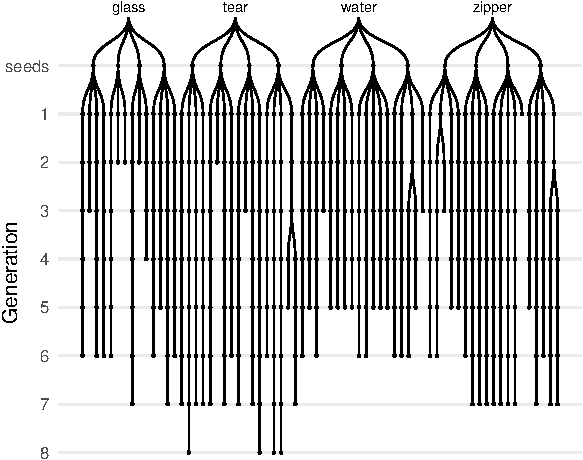
\includegraphics{fig1-1.pdf}
\caption{\label{fig:fig1}Vocal imitations collected in the transmission
chain experiment. Seed sounds (16) were sampled from four categories of
environmental sounds: glass, tear, water, zipper. Participants imitated
each seed sound, and then the next generation of participants imitated
the imitations, and so on, for up to 8 generations. Chains are
unbalanced due to random assignment and the exclusion of some low
quality recordings.}
\end{figure}

\hypertarget{measuring-acoustic-similarity}{%
\subsubsection{Measuring acoustic
similarity}\label{measuring-acoustic-similarity}}

Acoustic similarity judgments were obtained from five research
assistants who listened to pairs of sounds (approx. 300) and rated their
subjective similarity. On each trial, raters heard two sounds from
subsequent generations played in random order, and indicated the
similarity between the sounds on a 7- point Likert scale from
\emph{Entirely different and would never be confused} to \emph{Nearly
identical}. Full instructions and inter-rater reliability measures are
provided in the Supplemental Materials.

To obtain algorithmic measures of acoustic similarity, we used the
acoustic distance functions included in Phonological Corpus Tools
{[}39{]}. We computed Mel-frequency cepstral coefficients (MFCCs)
between pairs of imitations using 12 coefficients in order to obtain
speaker-independent estimates.

\hypertarget{collecting-transcriptions-of-imitations}{%
\subsubsection{Collecting transcriptions of
imitations}\label{collecting-transcriptions-of-imitations}}

Transcriptions were obtained for the first and last three generations of
each transmission chain. Additional \enquote{transcriptions} of the
original sounds used as seeds were also collected and are analyzed in
the Supplementary Materials (Fig. S6).

Participants (\emph{N}=216) recruited from Amazon Mechanical Turk were
paid to listen to imitations and write down what they heard as a single
\enquote{word} so that the written word would sound as much like the
sound as possible. Participants were instructed to avoid transcribing
the imitations into existing English words. Each participant completed
10 transcriptions.

\hypertarget{results}{%
\subsection{Results}\label{results}}

Imitations of environmental sounds became more stable over the course of
being repeated as revealed by increasing acoustic similarity judgments
along individual transmission chains. Acoustic similarity ratings were
fit with a linear mixed-effects model predicting perceived acoustic
similarity from generation with random effects (intercepts and slopes)
for raters. To test whether the hypothesized increase in acoustic
similarity was true across all seed sounds and categories, we added
random effects (intercepts and slopes) for seed sounds nested within
categories. The results showed that, across raters and seeds, imitations
from later generations were rated as sounding more similar to one
another than imitations from earlier generations, \emph{b} = 0.10 (SE =
0.03), \emph{t}(11.9) = 3.03, \emph{p} = 0.011 (Fig. 2). This result
suggests that imitations became more stable (i.e., easier to imitate
with high fidelity) with each generation of repetition.

\begin{figure}
\centering
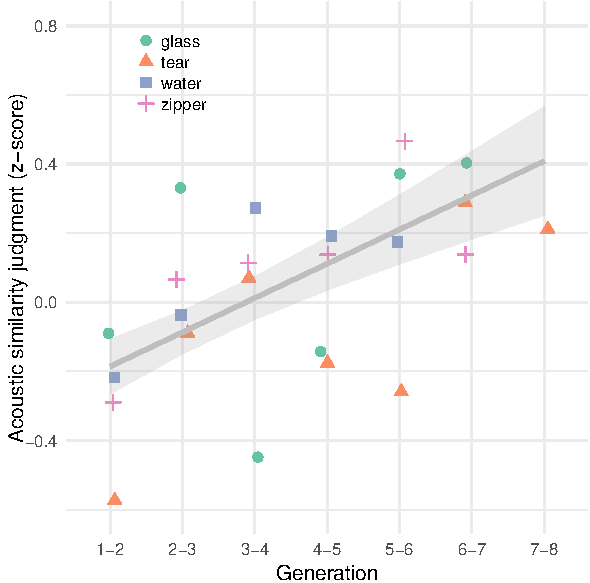
\includegraphics{fig2-1.pdf}
\caption{\label{fig:fig2}Change in perception of acoustic similarity over
generations of iterated imitation. Points depict mean acoustic
similarity ratings for pairs of imitations in each category. The
predictions of the linear mixed-effects model are shown with ±1 SE.}
\end{figure}

Increasing similarity along transmission chains could also reflect the
continuous degradation of the signal due to repeated imitation, in which
case acoustic similarity would increase both within as well as between
chains. To test this, we calculated MFCCs for pairs of sounds sampled
from within and between transmission chains across categories, and fit a
linear model predicting acoustic similarity from the generation of
sounds. We found that acoustic similarity increased within chains more
than it increased between chains, \emph{b} = -0.07 (SE = 0.03),
\emph{t}(6674.0) = -2.13, \emph{p} = 0.033 (Fig. S2), indicating that
imitations were stabilizing on divergent acoustic forms as opposed to
converging on similar forms through continuous degradation.

An additional test of stabilization and word-likeness was to measure
whether later generation imitations were transcribed more consistently
than first generation imitations. We collected a total of 2163
transcriptions --- approximately 20 transcriptions per sound. Of these,
179 transcriptions (8\%) were removed because they contained English
words. Some examples of the final transcriptions are presented in Table
1.

\begin{table}

\caption{\label{tab:table1}Examples of words transcribed from imitations.}
\centering
\begin{tabular}[t]{l|l|l}
\hline
Category & First generation & Last generation\\
\hline
glass & dirrng & wayew\\
\hline
tear & feeshefee & cheecheea\\
\hline
water & boococucuwich & galong\\
\hline
zipper & bzzzzup & izzip\\
\hline
\end{tabular}
\end{table}

To measure the similarity among transcriptions for a given imitation, we
calculated the average orthographic distance between the most frequent
transcription and all other transcriptions of the same imitation. We
then fit a hierarchical linear model predicting orthographic distance
from the generation of the imitation (First generation, Last generation)
with random effects (intercepts and slopes) for seed sound nested within
category. The results showed that transcriptions of last generation
imitations were more similar to one another than transcriptions of first
generation imitations, \emph{b} = -0.12 (SE = 0.03), \emph{t}(3.0) =
-3.62, \emph{p} = 0.035 (Fig. S3). The same result is reached through
alternative measures of orthographic distance (Fig. S4). Differences
between transcriptions of human vocalizations and transcriptions
directly of environmental sound cues are reported in the Supplementary
Materials (Fig. S6).

\hypertarget{discussion}{%
\subsection{Discussion}\label{discussion}}

Repeating imitations of environmental sounds over generations of
imitators was sufficient to create more word-like forms, even without
any explicit intent to communicate. We defined word-likeness in terms of
acoustic stability and orthographic agreement. With each repetition, the
acoustic forms of the imitations became more similar to one another,
indicating they became easier to repeat with high fidelity. The
possibility that this similarity was due to uniform degradation across
all transmission chains was ruled out by algorithmic analyses of
acoustic similarity demonstrating that acoustic similarity increased
within chains but not between them. Additionally, later generation
imitations were transcribed more consistently into English orthography,
further supporting our hypothesis that repeating imitations makes them
more stable and word-like.

The results of Experiment 1 demonstrate the ease with which iterated
imitation gives rise to stable wordforms. However, the results do not
address how these emergent words relate to the original sounds that were
being imitated. As the imitations became more word-like, were they
stabilizing on arbitrary acoustic and orthographic forms, or did they
maintain some resemblance to the environmental sounds that motivated
them? The purpose of Experiment 2 was to assess the extent to which
repeated imitations and their transcriptions maintained a resemblance to
the original set of seed sounds.

\hypertarget{experiment-2-resemblance-of-imitations-to-original-seed-sounds}{%
\section{Experiment 2: Resemblance of imitations to original seed
sounds}\label{experiment-2-resemblance-of-imitations-to-original-seed-sounds}}

To assess the resemblance of repeated imitations to the original seed
sounds, we measured the ability of participants naïve to the design of
the experiment to match imitations and their transcriptions back to
their original sound source relative to other seed sounds from either
the same category or from different categories (Fig. 3A). Using these
match accuracies, we first asked whether and for how many generations
the imitations and their transcriptions could be matched back to the
original sounds. Second, we asked whether repeated imitation resulted in
a uniform degradation of the signal in each imitation, or if repeated
imitation resulted in some kinds of information degrading more rapidly
than others. Specifically, we tested the hypothesis that if imitations
were becoming more word-like, then they should also be interpreted more
categorically, and thus we anticipated that imitations would lose
information identifying the specific source of an imitation more rapidly
than category information that identifies the category of environmental
sound being imitated.

\hypertarget{methods-1}{%
\subsection{Methods}\label{methods-1}}

\hypertarget{matching-imitations-to-seed-sounds}{%
\subsubsection{Matching imitations to seed
sounds}\label{matching-imitations-to-seed-sounds}}

Participants (\emph{N}=751) recruited from Amazon Mechanical Turk were
paid to listen to imitations, one at a time, and for each one, choose
one of four possible sounds they thought the person was trying to
imitate. The task was not speeded and no feedback was provided.
Participants completed 10 questions at a time.

All imitations were tested in each of the three question types depicted
in Fig. 3A. These questions differed in the relationship between the
imitation and the four seed sounds provided as the choices in the
question. Question types (True seed, Category match, Specific match)
were assigned between-subject.

\hypertarget{matching-transcriptions-to-seed-sounds}{%
\subsubsection{Matching transcriptions to seed
sounds}\label{matching-transcriptions-to-seed-sounds}}

Participants (\emph{N}=461) recruited from Amazon Mechanical Turk
completed a modified version of the matching survey described above.
Instead of listening to imitations, participants now read a word (a
transcription of an imitation), which they were told was invented to
describe one of the four presented sounds. Of the unique transcriptions
that were generated for each sound (imitations and seed sounds), only
the top four most frequent transcriptions were used in the matching
experiment. The distractors for all questions were between-category,
i.e.~true seed and category match. Specific match questions were
omitted.

\hypertarget{results-1}{%
\subsection{Results}\label{results-1}}

Response accuracies in matching imitations to seed sounds were fit by a
generalized linear mixed-effects model predicting match accuracy as
different from chance (25\%) based on the type of question being
answered (True seed, Category match, Specific match) and the generation
of the imitation. Question types were contrast coded using Category
match questions as the baseline condition in comparison to the other two
question types, each containing the actual seed that generated the
imitation as one of the choices. The model included random intercepts
for participant, and random slopes and intercepts for seed sounds nested
within categories.

Accuracy in matching first generation imitations to seed sounds was
above chance for all question types, \emph{b} = 1.65 (SE = 0.14)
log-odds, odds = 0.50, \emph{z} = 11.58, \emph{p} \textless{} 0.001, and
decreased steadily over generations, \emph{b} = -0.16 (SE = 0.04)
log-odds, \emph{z} = -3.72, \emph{p} \textless{} 0.001. We then tested
whether this increase in difficulty was constant across the three types
of questions or if some question types became more difficult than
others. The results are shown in Fig. 3B. Performance decreased over
generations more rapidly for questions requiring a within-category
distinction than for between-category questions, \emph{b} = -0.08 (SE =
0.03) log-odds, \emph{z} = -2.68, \emph{p} = 0.007, suggesting that
between-category information was more resistant to loss through repeated
imitation.

An alternative explanation of the drop off in accuracy for
within-category questions but not category match questions is that the
within-category questions are simply more difficult because the sounds
presented as choices are more acoustically similar to one another.
However, performance also decreased relative to the category match
questions for the easiest type of question where the correct answer was
the actual seed generating the imitation (True seed questions; see Fig.
3A). That is, the advantage of having the true seed among
between-category distractors decreased over generations, \emph{b} =
-0.07 (SE = 0.02) log-odds, \emph{z} = -2.77, \emph{p} = 0.006. The
observed decrease in the \enquote{true seed advantage} (the advantage of
having the actual seed among the choices) combined with the increase in
the \enquote{category advantage} (the advantage of having
between-category distractors) shows that the changes induced by repeated
imitation caused the imitations to lose some of properties that linked
the earlier imitations to the specific sound that motivated them, while
nevertheless preserving a more abstract category-based resemblance.

We next report the results of matching the written transcriptions of the
auditory sounds back to the original environmental sounds. Remarkably,
participants were able to guess the correct meaning of a word that was
transcribed from an imitation that had been repeated up to 8 times,
\emph{b} = 0.83 (SE = 0.13) log-odds, odds = -0.18, \emph{z} = 6.46,
\emph{p} \textless{} 0.001 (Fig. 3C). This was true for True seed
questions containing the actual seed generating the transcribed
imitation, \emph{b} = 0.75 (SE = 0.15) log-odds, \emph{z} = 4.87,
\emph{p} \textless{} 0.001, and for Category match questions where
participants had to associate transcriptions with a particular category
of environmental sounds, \emph{b} = 1.02 (SE = 0.16) log-odds, \emph{z}
= 6.39, \emph{p} \textless{} 0.001. The effect of generation did not
vary across these question types, \emph{b} = 0.05 (SE = 0.10) log-odds,
\emph{z} = 0.47, \emph{p} = 0.638. The results of matching
\enquote{transcriptions} directly of the environmental sounds are shown
in Fig. S6.

\begin{figure}
\centering
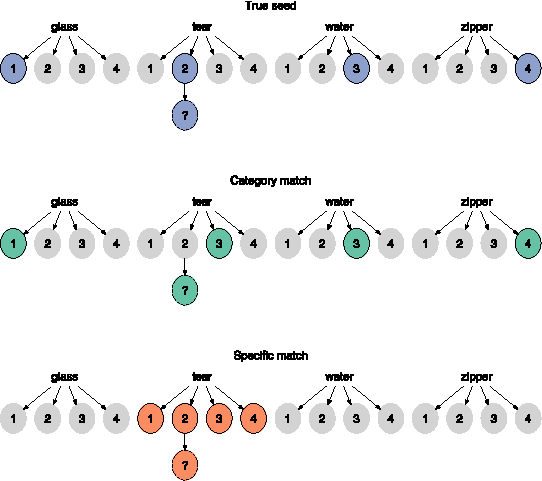
\includegraphics{fig3-1.pdf}
\caption{\label{fig:fig3}Repeated imitations retained category resemblance.
A. Three types of matching questions. True seed and category match
questions had choices from different sound categories. Specific match
questions pitted the actual seed against the other seeds within the same
category. B. Accuracy in matching vocal imitations to original seed
sounds. Curves show predictions of the generalized linear mixed effects
models with ±1 SE of the model predictions. C. Accuracy in matching
transcriptions of the imitations to original seed sounds (e.g.,
\enquote{boococucuwich} to a water splashing sound). Circles show mean
matching accuracy for the vocal imitations that were transcribed for
comparison.}
\end{figure}

\hypertarget{discussion-1}{%
\subsection{Discussion}\label{discussion-1}}

Even after being repeated up to 8 times across 8 different individuals,
vocalizations retained a resemblance to the environmental sound that
motivated them. This resemblance remained even after the vocalizations
were transcribed into orthographic forms. For vocal imitations, but not
for transcriptions, this resemblance was stronger for the category of
environmental sound than the actual seed sound, suggesting that iterated
imitation produces vocalizations that are interpreted by naïve listeners
in a more categorical way. Iterated imitation appears to strip the
vocalizations of some of the characteristics that individuate each
particular sound while maintaining some category-based resemblance (even
though participants were never informed about the meaning of the
vocalizations and were not trying to communicate).

Transcriptions of the vocalizations, like the vocalizations themselves,
were able to be matched to the original environmental sounds at levels
above chance. Unlike vocalizations, the transcriptions continued to be
matched more accurately to the true seed compared to the general
category. That is, transcription appears to impact specific and
category-level information equally. One possible explanation of the
difference between the acoustic and orthographic forms of this task is
that the process of transcribing a non- linguistic vocalization into a
written word encourages transcribers to emphasize individuating
information about the vocalization. However, the fact that
transcriptions of imitations can be matched back to other category
members (Category match questions) suggests that transcriptions still
carry some category information, so this is not a complete explanation
of our results. Another possible reason is that by selecting only the
most frequent transcriptions, we unintentionally excluded less frequent
transcriptions that were nonetheless more diagnostic of category
information.

Experiments 1 and 2 document a process of gradual change from an
imitation of an environmental sound to a more word-like form. But do
these emergent words function like other words in the language? In
Experiment 3, we test the suitability of words taken from the beginning
and end of transmission chains in serving as category labels in a
category learning task.

\hypertarget{experiment-3-suitability-of-created-words-as-category-labels}{%
\section{Experiment 3: Suitability of created words as category
labels}\label{experiment-3-suitability-of-created-words-as-category-labels}}

One consequence of imitations becoming more word-like is that they may
make for better category labels. For example, an imitation from a later
generation, by virtue of having a more word-like form, may be easier to
learn as a label for the category of sounds that motivated it than an
earlier imitation, which is more closely yoked to a particular
environmental sound. To the extent that repeating imitations abstracts
away the idiosyncrasies of a particular category member {[}40,41{]}, it
may also be easier to generalize to new category members. We tested
these predictions using a category learning task in which participants
learned novel labels for the categories of environmental sounds. The
novel labels were transcriptions of either first or last generation
imitations gathered in Experiment 1.

\hypertarget{methods-2}{%
\subsection{Methods}\label{methods-2}}

\hypertarget{selecting-words-to-learn-as-category-labels}{%
\subsubsection{Selecting words to learn as category
labels}\label{selecting-words-to-learn-as-category-labels}}

Of the 1814 unique words created through the transmission chain and
transcription procedures, we sampled 56 words transcribed from first and
last generation imitations that were equated in terms of length and
match accuracy with the original sounds. Our procedure for selecting
otherwise-equal transcriptions is detailed in the Supplementary
Materials.

\hypertarget{procedure}{%
\subsubsection{Procedure}\label{procedure}}

Participants (\emph{N}=67) were University of Wisconsin undergraduates
who received course credit for participation. Participants were randomly
assigned four novel labels to learn for four categories of environmental
sounds. Full instructions are provided in the Supplementary Materials.
Participants were assigned between-subject to learn labels
(transcriptions) of either first or last generation imitations. On each
trial, participants heard one of the 16 seed sounds. After a 1s delay,
participants saw a label (one of the transcribed imitations) and
responded yes or no using a gamepad controller depending on whether the
sound and the word went together. Participants received accuracy
feedback (a bell sound and a green checkmark if correct; a buzzing sound
and a red \enquote{X} if incorrect). Four outlier participants were
excluded from the final sample due to high error rates and slow RTs.

Participants categorized all 16 seed sounds over the course of the
experiment, but they learned them in blocks of 4 sounds at a time.
Within each block of 24 trials, participants heard the same four sounds
and the same four words multiple times, with a 50\% probability of the
sound matching the word on any given trial. At the start of a new block
of trials, participants heard four new sounds they had not heard before,
and had to learn to associate these new sounds with the words they had
learned in the previous blocks.

\hypertarget{results-2}{%
\subsection{Results}\label{results-2}}

Participants began by learning through trial-and-error to associate four
written labels with four categories of environmental sounds. The small
number of categories made this an easy task (mean accuracy after the
first block of 24 trials was 81\%; Fig. S5). Participants learning
transcriptions of first or last generation imitations did not differ in
overall accuracy, \emph{p} = 0.887, or reaction time, \emph{p} = 0.616.

After this initial learning phase (i.e.~after the first block of
trials), accuracy performance quickly reached ceiling and did not differ
between groups \emph{p} = 0.775. However, the response times of
participants learning last generation transcriptions declined more
rapidly with practice than participants learning first generation
transcriptions, \emph{b} = -114.13 (SE = 52.06), \emph{t}(39.9) = -2.19,
\emph{p} = 0.034 (Fig. 4A). These faster responses suggest that, in
addition to becoming more stable both in terms of acoustic and
orthographic properties, repeating imitations makes them easier to
process as category labels. We predict that given a harder task (i.e.,
more than four categories and 16 exemplars) would yield differences in
initial learning rates as well.

Next, we examined whether transcriptions from last generation imitations
were easier to generalize to novel category exemplars. To test this
hypothesis, we compared RTs on trials immediately prior to the
introduction of novel sounds (new category members) and the first trials
after the block transition (±6 trials). The results revealed a reliable
interaction between the generation of the transcribed imitation and the
block transition, \emph{b} = -110.77 (SE = 52.84), \emph{t}(39.7) =
-2.10, \emph{p} = 0.042 (Fig. 4B). This result suggests that
transcriptions from later generation imitations were easier to
generalize to new category members.

\begin{figure}
\centering
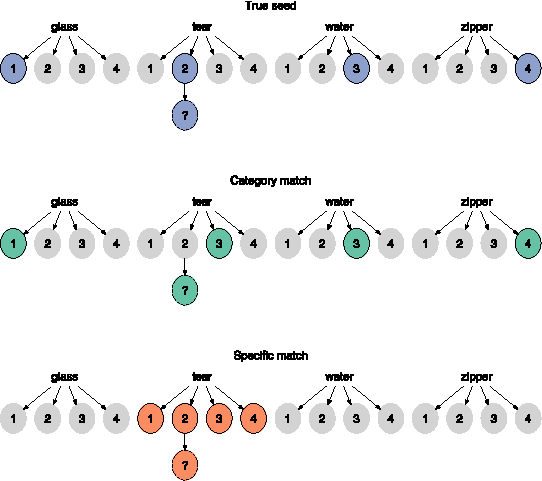
\includegraphics{fig4-1.pdf}
\caption{\label{fig:fig4}Repeated imitations made for better category
labels. A. Mean RTs for correct responses in the category learning
experiment with ±1 SE. B. Cost of generalizing to new category members
with ±1 SE.}
\end{figure}

\hypertarget{discussion-2}{%
\subsection{Discussion}\label{discussion-2}}

The results of a simple category learning experiment demonstrate a
possible benefit to the stabilization of repeated imitations on more
word-like forms. As a consequence of being more word-like, repeated
imitations were responded to more quickly, and generalized to new
category members more easily. These results suggest an advantage to
repeating imitations from the perspective of the language learner in
that they afford better category generalization.

\hypertarget{general-discussion}{%
\section{General Discussion}\label{general-discussion}}

Accumulating evidence shows that iconic words are prevalent across the
spoken languages of the world {[}25,26,32{]}. And counter to past
assumptions about the limitations of human vocal imitation, people are
surprisingly effective at using vocal imitation to represent and
communicate about the sounds in their environment {[}35{]} and more
abstract meanings {[}33{]}. These findings raise the hypothesis that
early spoken words originated from vocal imitations, perhaps comparable
to the way that many of the signs of signed languages appear to be
formed originally from pantomimes {[}33,42{]}. Here, we examined whether
simply repeating an imitation of an environmental sound --- with no
intention to create a new word or even to communicate --- produces more
word-like forms.

Our results show that through unguided repetition, imitative
vocalizations became more word-like both in form and function. In form,
the vocalizations gradually stabilized over generations, becoming more
similar from imitation to imitation. The standardization was also found
when the words were transcribed into the English alphabet. Even as the
vocalizations became more word-like, they maintained a resemblance to
the original environmental sounds that motivated them. Notably, this
resemblance appeared to be greater with respect to the category of sound
(e.g., water-splashing sounds), rather than to the specific exemplar (a
particular water-splashing sound). After eight generations the
vocalizations could no longer be matched to the particular sound from
which they originated any more accurately than they could be matched to
the general category of environmental sound. Thus, information that
distinguished an imitation from other sound categories was more
resilient to transmission decay than exemplar information within a
category. Remarkably, the resemblance to the original sounds was
maintained even when the vocalizations were transcribed into a written
form: participants were able to match the transcribed vocalizations to
the original sound category at levels above chance.

We further tested the hypothesis that repeated imitation led to
vocalizations becoming more word-like by testing the ease with which
people learned the (transcribed) vocalizations as category labels (e.g.,
\enquote{pshfft} from generation 1 vs. \enquote{shewp} from generation 8
as labels for tearing sounds) (Exp. 3). Labels from the last generation
were responded to more quickly than labels from the first generation.
More importantly the labels from the last generation generalized better
to novel category members. This fits with previous research showing that
the relatively arbitrary forms that are typical of words (e.g.
\enquote{dog}) makes them better suited to function as category labels
compared to direct auditory cues (e.g., the sound of a dog bark)
{[}40,41,43{]}.

Even as the vocalizations became more word-like, they nevertheless
maintained an imitative quality. After eight generations they could no
longer be matched to the particular sound from which they originated any
more accurately than they could be matched to the general category of
environmental sound. Thus, information that distinguished an imitation
from other sound categories was more resilient to transmission decay
than exemplar information within a category. Remarkably, even after the
vocalizations were transcribed into English orthography, participants
were able to guess their original sound category from the written
\enquote{words}. In contrast to the vocalizations, participants
continued to be more accurate at matching late generation transcriptions
back to their particular source sound relative to other exemplars from
the same category.

Unlike the large number of iconic signs in signed languages {[}10{]},
the number of iconic words in spoken languages may appear to be very
small {[}44,45{]}. However, increasing evidence from disparate language
suggests that vocal imitation is, in fact, a widespread source of
vocabulary. Cross-linguistic surveys indicate that onomatopoeia---iconic
words used to represent sounds---are a universal lexical category found
across the world's languages {[}46{]}. Even English, a language that has
been characterized as relatively limited in iconic vocabulary {[}47{]},
is documented as having hundreds of onomatopoeic words not only for
animal and human vocalizations (\enquote{meow}, \enquote{tweet},
\enquote{slurp}, \enquote{babble}, murmur''), but also for a variety of
environmental sounds (e.g., \enquote{ping}, \enquote{click},
\enquote{plop}) {[}36,48{]}. Besides words that directly resemble sounds
--- the focus of the present study --- many languages contain
semantically broader inventories of ideophones. These words comprise a
grammatically and phonologically distinct class of words that are used
to express various sensory-rich meanings, such as qualities related to
manner of motion, visual properties, textures and touch, inner feelings
and cognitive states {[}46,49,50{]}. As with onomatopoeia, ideophones
are often recognized by naïve listeners as bearing a degree of
resemblance to their meaning {[}51{]}.

Our study focused on imitations of environmental sounds, and more work
remains to be done to determine the extent to which vocal imitation can
ground de novo vocabulary creation in other semantic domains
{[}33,52{]}. Notably, our hypothesis that vocal imitation may have
played a role in the origin of some of the first spoken words does not
preclude that gesture played an equal or more important role in
establishing the first linguistic conventions {[}10,11,53{]}. What the
present results make clear is that the transition from imitation to word
can be a rapid and simple process: the mere act of repeated imitation
can drive vocalizations to become more word-like in both form and
function while still retaining some resemblance to the real world
referents.

\hypertarget{ethics}{%
\section{Ethics}\label{ethics}}

This was approved by the University of Wisconsin-Madison's Educational
and Social/Behavioral Sciences Institutional Review Board and conducted
in accordance with the principles expressed in the Declaration of
Helsinki. Informed consent was obtained for all participants.

\hypertarget{data-code-and-materials}{%
\section{Data, code, and materials}\label{data-code-and-materials}}

Our data along with all methods, materials, and analysis scripts, are
available in public repositories described on the Open Science Framework
page for this research here: \href{https://osf.io/3navm}{osf.io/3navm}.

\hypertarget{competing-interests}{%
\section{Competing interests}\label{competing-interests}}

We have no competing interests.

\hypertarget{authors-contributions}{%
\section{Authors' contributions}\label{authors-contributions}}

P.E., M.P., and G.L. designed the research. P.E. conducted the research
and analyzed the data. P.E., M.P., and G.L. wrote the manuscript.

\hypertarget{funding}{%
\section{Funding}\label{funding}}

This research was supported by NSF 1344279 awarded to G.L.

\hypertarget{references}{%
\section{References}\label{references}}

\setlength{\parindent}{-0.5in}\setlength{\leftskip}{0.5in}

\hypertarget{refs}{}
\leavevmode\hypertarget{ref-Seyfarth:1986tw}{}%
1. Seyfarth RM, Cheney DL. 1986 Vocal development in vervet monkeys.
\emph{Animal Behaviour} \textbf{34}, 1640--1658.

\leavevmode\hypertarget{ref-Crockford:2004cz}{}%
2. Crockford C, Herbinger I, Vigilant L, Boesch C. 2004 Wild chimpanzees
produce group-specific calls: a case for vocal learning? \emph{Ethology}
\textbf{110}, 221--243.

\leavevmode\hypertarget{ref-Brysbaert:2016fg}{}%
3. Brysbaert M, Stevens M, Mandera P, Keuleers E. 2016 How Many Words Do
We Know? Practical Estimates of Vocabulary Size Dependent on Word
Definition, the Degree of Language Input and the Participant's Age.
\emph{Frontiers in Psychology} \textbf{7}, 55--11.

\leavevmode\hypertarget{ref-Wierzbicka:1996sm}{}%
4. Wierzbicka A. 1996 \emph{Semantics: Primes and universals: Primes and
universals}. Oxford University Press, UK.

\leavevmode\hypertarget{ref-Evans:2009dk}{}%
5. Evans N, Levinson SC. 2009 The myth of language universals: Language
diversity and its importance for cognitive science. \emph{Brain and
Behavioral Sciences} \textbf{32}, 429--492.

\leavevmode\hypertarget{ref-Lupyan:2016uw}{}%
6. Lupyan G, Dale R. 2016 Why are there different languages? The role of
adaptation in linguistic diversity.

\leavevmode\hypertarget{ref-Pagel:2007br}{}%
7. Pagel M, Atkinson QD, Meade A. 2007 Frequency of word-use predicts
rates of lexical evolution throughout Indo-European history.
\emph{Nature} \textbf{449}, 717--720.

\leavevmode\hypertarget{ref-Sapir:1921}{}%
8. Sapir E. 1921 \emph{Language: An introduction to the study of
speech}. New York: Harcourt, Brace; Company.

\leavevmode\hypertarget{ref-Labov:1972}{}%
9. Labov W. 1972 \emph{Sociolinguistic patterns}. University of
Pennsylvania Press.

\leavevmode\hypertarget{ref-GoldinMeadow:2016bw}{}%
10. Goldin-Meadow S. 2016 What the hands can tell us about language
emergence. \emph{Psychonomic Bulletin \& Review} \textbf{24}, 1--6.

\leavevmode\hypertarget{ref-Kendon:2014eg}{}%
11. Kendon A. 2014 Semiotic diversity in utterance production and the
concept of 'language'. \emph{Philosophical Transactions of the Royal
Society B: Biological Sciences} \textbf{369}, 20130293--20130293.

\leavevmode\hypertarget{ref-Klima:1980si}{}%
12. Klima ES, Bellugi U. 1980 \emph{The signs of language}. Harvard
University Press.

\leavevmode\hypertarget{ref-Frishberg:1975dh}{}%
13. Frishberg N. 1975 Arbitrariness and Iconicity: Historical Change in
American Sign Language. \emph{Language} \textbf{51}, 696--719.

\leavevmode\hypertarget{ref-Stokoe:1965}{}%
14. Stokoe W. 1965 \emph{Dictionary of the American Sign Language based
on scientific principles}. Gallaudet College Press, Washington.

\leavevmode\hypertarget{ref-Wescott:1971to}{}%
15. Wescott RW. 1971 Linguistic iconism. \emph{Linguistic Society of
America} \textbf{47}, 416--428.

\leavevmode\hypertarget{ref-GoldinMeadow:1977gz}{}%
16. Goldin-Meadow S, Feldman H. 1977 The development of language-like
communication without a language model. \emph{Science} \textbf{197},
401--403.

\leavevmode\hypertarget{ref-Fay:2014cw}{}%
17. Fay N, Lister CJ, Ellison TM, Goldin-Meadow S. 2014 Creating a
communication system from scratch: Gesture beats vocalization hands
down. \emph{Frontiers in Psychology} \textbf{5}, 663.

\leavevmode\hypertarget{ref-Arbib:2012htb}{}%
18. Arbib MA. 2012 \emph{How the brain got language: The mirror system
hypothesis}. Oxford University Press.

\leavevmode\hypertarget{ref-Armstrong:2007go}{}%
19. Armstrong DF, Wilcox S. 2007 \emph{The gestural origin of language}.
Oxford University Press.

\leavevmode\hypertarget{ref-Corballis:2003ha}{}%
20. Corballis MC. 2003 \emph{From hand to mouth: The origins of
language}. Princeton University Press.

\leavevmode\hypertarget{ref-Hewes:1973vr}{}%
21. Hewes GW. 1973 Primate Communication and the Gestural Origin of
Language. \emph{Current Anthropology} \textbf{14}, 5--24.

\leavevmode\hypertarget{ref-Hockett:1978se}{}%
22. Hockett CF. 1978 In search of Jove's brow. \emph{American speech}
\textbf{53}, 243--313.

\leavevmode\hypertarget{ref-Tomasello:2010or}{}%
23. Tomasello M. 2010 \emph{Origins of human communication}. MIT press.

\leavevmode\hypertarget{ref-Pinker:2005cv}{}%
24. Pinker S, Jackendoff R. 2005 The faculty of language: what's special
about it? \emph{Cognition} \textbf{95}, 201--236.

\leavevmode\hypertarget{ref-Dingemanse:2015cu}{}%
25. Dingemanse M, Blasi DE, Lupyan G, Christiansen MH, Monaghan P. 2015
Arbitrariness, Iconicity, and Systematicity in Language. \emph{Trends in
Cognitive Sciences} \textbf{19}, 603--615.

\leavevmode\hypertarget{ref-Perniss:2010fb}{}%
26. Perniss P, Thompson RL, Vigliocco G. 2010 Iconicity as a General
Property of Language: Evidence from Spoken and Signed Languages.
\emph{Frontiers in Psychology} \textbf{1}.

\leavevmode\hypertarget{ref-Clark:1990cl}{}%
27. Clark HH, Gerrig RJ. 1990 Quotations as demonstrations.
\emph{Language} \textbf{66}, 764--805.

\leavevmode\hypertarget{ref-Lewis:2009wz}{}%
28. Lewis J. 2009 As well as words: Congo Pygmy hunting, mimicry, and
play. In \emph{The cradle of language}, The cradle of language.

\leavevmode\hypertarget{ref-Brown:1955wy}{}%
29. Brown RW, Black AH, Horowitz AE. 1955 Phonetic symbolism in natural
languages. \emph{Journal of abnormal psychology} \textbf{50}, 388--393.

\leavevmode\hypertarget{ref-Dingemanse:2014gj}{}%
30. Dingemanse M. 2014 Making new ideophones in Siwu: Creative depiction
in conversation. \emph{Pragmatics and Society}

\leavevmode\hypertarget{ref-Donald:2016kd}{}%
31. Donald M. 2016 Key cognitive preconditions for the evolution of
language. \emph{Psychonomic Bulletin \& Review}, 1--5.

\leavevmode\hypertarget{ref-Imai:2014dea}{}%
32. Imai M, Kita S. 2014 The sound symbolism bootstrapping hypothesis
for language acquisition and language evolution. \emph{Philosophical
Transactions of the Royal Society B: Biological Sciences} \textbf{369}.

\leavevmode\hypertarget{ref-Perlman:2015ip}{}%
33. Perlman M, Dale R, Lupyan G. 2015 Iconicity can ground the creation
of vocal symbols. \emph{Royal Society Open Science} \textbf{2},
150152--16.

\leavevmode\hypertarget{ref-Lemaitre:2014kr}{}%
34. Lemaitre G, Rocchesso D. 2014 On the effectiveness of vocal
imitations and verbal descriptions of sounds. \emph{The Journal of the
Acoustical Society of America} \textbf{135}, 862--873.

\leavevmode\hypertarget{ref-Lemaitre:2016kz}{}%
35. Lemaitre G, Houix O, Voisin F, Misdariis N, Susini P. 2016 Vocal
Imitations of Non-Vocal Sounds. \emph{PloS one} \textbf{11},
e0168167--28.

\leavevmode\hypertarget{ref-Rhodes:1994au}{}%
36. Rhodes R. 1994 Aural images. \emph{Sound symbolism}, 276--292.

\leavevmode\hypertarget{ref-Tamariz:2017bd}{}%
37. Tamariz M. 2017 Experimental Studies on the Cultural Evolution of
Language. \emph{Annual Review of Linguistics} \textbf{3}, 389--407.

\leavevmode\hypertarget{ref-Kirby:2008kja}{}%
38. Kirby S, Cornish H, Smith K. 2008 Cumulative cultural evolution in
the laboratory: an experimental approach to the origins of structure in
human language. \emph{Proceedings of the National Academy of Sciences}
\textbf{105}, 10681--10686.

\leavevmode\hypertarget{ref-PCT:1.1}{}%
39. Hall KC, Allen B, Fry M, Mackie S, McAuliffe M. 2016 Phonological
CorpusTools. \emph{14th Conference for Laboratory Phonology}

\leavevmode\hypertarget{ref-Edmiston:2015he}{}%
40. Edmiston P, Lupyan G. 2015 What makes words special? Words as
unmotivated cues. \emph{Cognition} \textbf{143}, 93--100.

\leavevmode\hypertarget{ref-Lupyan:2012cp}{}%
41. Lupyan G, Thompson-Schill SL. 2012 The evocative power of words:
Activation of concepts by verbal and nonverbal means. \emph{Journal of
Experimental Psychology: General} \textbf{141}, 170--186.

\leavevmode\hypertarget{ref-Fay:2014ih}{}%
42. Fay N, Ellison TM, Garrod S. 2014 Iconicity: From sign to system in
human communication and language. \emph{Pragmatics and Cognition}
\textbf{22}, 244--263.

\leavevmode\hypertarget{ref-Boutonnet:2015fz}{}%
43. Boutonnet B, Lupyan G. 2015 Words Jump-Start Vision: A Label
Advantage in Object Recognition. \emph{Journal of Neuroscience}
\textbf{35}, 9329--9335.

\leavevmode\hypertarget{ref-Crystal:1987en}{}%
44. Crystal D. 1987 \emph{The Cambridge Encyclopedia of Language}.
Cambridge Univ Press.

\leavevmode\hypertarget{ref-Newmeyer:1992we}{}%
45. Newmeyer FJ. 1992 Iconicity and generative grammar. \emph{Language}

\leavevmode\hypertarget{ref-Dingemanse:2012fc}{}%
46. Dingemanse M. 2012 Advances in the Cross-Linguistic Study of
Ideophones. \emph{Language and Linguistics Compass} \textbf{6},
654--672.

\leavevmode\hypertarget{ref-Vigliocco:2014fc}{}%
47. Vigliocco G, Perniss P, Vinson D. 2014 Language as a multimodal
phenomenon: implications for language learning, processing and
evolution. \emph{Philosophical Transactions of the Royal Society B:
Biological Sciences} \textbf{369}, 20130292--20130292.

\leavevmode\hypertarget{ref-Sobkowiak:1990ph}{}%
48. Sobkowiak W. 1990 On the phonostatistics of English onomatopoeia.
\emph{Studia Anglica Posnaniensia} \textbf{23}, 15--30.

\leavevmode\hypertarget{ref-Nuckolls:1999ca}{}%
49. Nuckolls JB. 1999 The case for sound symbolism. \emph{Annual Review
of Anthropology} \textbf{28}, 225--252.

\leavevmode\hypertarget{ref-Voeltz:2001vv}{}%
50. Voeltz FE, Kilian-Hatz C. 2001 \emph{Ideophones}. John Benjamins
Publishing.

\leavevmode\hypertarget{ref-Dingemanse:2016vd}{}%
51. Dingemanse M, Schuerman W, Reinisch E. 2016 What sound symbolism can
and cannot do: Testing the iconicity of ideophones from five languages.
\emph{Language} \textbf{92}.

\leavevmode\hypertarget{ref-Lupyan:2015vic}{}%
52. Lupyan G, Perlman M. 2015 The vocal iconicity challenge! In
\emph{The th biennial protolanguage conference}, Rome, Italy.

\leavevmode\hypertarget{ref-Fay:2013jpa}{}%
53. Fay N, Arbib MA, Garrod S. 2013 How to Bootstrap a Human
Communication System. \emph{Cognitive Science} \textbf{37}, 1356--1367.


\clearpage
\renewcommand{\listtablename}{Table captions}
\listoftables

\clearpage
\renewcommand{\listfigurename}{Figure captions}
\listoffigures



\end{document}
